




\section{Projekt- und Programmstruktur}
\subsection{Interpretation binärer Zahlen}
 Matlab fi
 
 immer 10 Nachkommastellen, außer bei Multiplikation
 
 NC Sim, nur Integerdarstellung möglich, bei Vektoren sogar nur positiv
 
 \subsection{Struktureller Aufbau}
 Konstanten
 
 Datentypen
 
 readfile (read\_input\_matrix) 
 
 writefile (write\_results)
 
 resize-Funktion
 
 \subsection{Bibliotheken}
\texttt{library ieee;}

\texttt{use ieee.std\_logic\_1164.all;}

\texttt{use ieee.numeric\_std.all;}

\texttt{use ieee.std\_logic\_arith.all;}

\texttt{use ieee.std\_logic\_unsigned.all;}


\texttt{library STD;}

\texttt{use STD.TEXTIO.ALL;}

\texttt{use ieee.std\_logic\_textio.all;}



VHDL 2008 kann auch Kommazahlen darstellen ( signed fixed : sfixed(2 downto -10) )




\section{Entwicklungsstufen}

\subsection{2D-DFT-Implementierung in VHDL}

In Tabelle \ref{tab:TakteKomplexeDFT} ist eine Auflistung der für die Berechnung veranschlagten Takte für die Multiplikation einer beliebigen Matrix mit der
Twiddlefaktormatrix für die 8x8-DFT zu sehen. Grundlage ist, dass in einem Takt Summanden 
paarweise aufaddiert werden und in einer Variablen zwischengespeichert werden. Dieses Verfahren kann auch als Baumstruktur aufgefasst werden. 
Wie das Aufsummieren erfolgt, kann in Abschnitt \ref{sec:Berechnungsschema} detaillierter nachgelesen werden.

Wie in Abschnitt \ref{sec:Konstantenmultiplizierer} gezeigt wird, kann die Multiplikation mit einer Konstanten innerhalb eines Taktes mit einem Schaltnetz erfolgen. 

In Abschnitt \ref{sec:Syntheseergebnisse} wird gezeigt, dass der kritische Pfad der Negierung sogar etwas länger als beim Konstantenmultiplizierer ist.
Um keine zu langen Signal- und Gatterlaufzeiten hervorzurufen, sollte hierfür unbedingt ein eigener Takt eingeplant werden. Dadurch relativiert sich der zeitliche Gewinn allerdings 
etwas. 


\begin{table}[htbp]
\centering
\caption{Takte für die komplexe DFT}
\label{tab:TakteKomplexeDFT}
\begin{tabular}{ccccc}
\hline
\multirow{2}{*}{Zeile} & Additionen & Takte pro Element & Takte für & Summe der\\
      & pro Element ($N$) & ($\log_2(N)$) & Multiplikation & Takte\\
\hline
 1& 8  & 3   &0 &3\\
 2& 12 & 3,6 &1 &5\\
 3& 8  & 3   &0 &3\\
 4& 12 & 3,6 &1 &5\\
 5& 8  & 3   &0 &3\\
 6& 12 & 3,6 &1 &5\\
 7& 8  & 3   &0 &3\\
 8& 12 & 3,6 &1 &5\\
\hline
\end{tabular}
\end{table}

Anhand der rechten Spalte ergeben sich so (3+5)$\cdot$4$\cdot$8 = 256 Takte sowohl für den Real- als auch den Imaginärteil der komplexen Ausgangsmatrix. Real- und Imaginärteil
werden parallel berechnet und sind somit zeitgleich fertig.


\subsection{Weiterentwickelung zur 2D-DFT}

Ziel ist es die gleiche DFT-Einheit für beide DFTs zu verwenden

Zähler für 64 Werte kann als 6 Bit Vektor realisiert werden, der bei 63 einen Überlauf hat und wieder bei 0 anfängt.

Vorderen 3 Bit sind die der Zeile, die hinteren für die Spalte.

Das dritte Bit von vorne sagt einem, ob es eine gerade oder ungerade Zeile ist.


 
 
 
Die in Gleichung (\ref{eq:2D-DFT_MatrixMult}) beschriebene Berechnung der 2D-DFT lässt sich auch wie folgt schreiben:

\begin{align}
 X &= W \cdot x \cdot W \nonumber \\
   &= \left(x^T\cdot W\right)^T\cdot W \label{eq:MatMultTranspose1} \\
   &= X^* \cdot W \nonumber\\
   &= \left(\left(x\cdot W\right)^T\cdot W\right)^T \label{eq:MatMultTranspose2}\\
   &= \left(X^{*T} \cdot W\right)^T \nonumber
\end{align}

In Matlab muss hierfür entweder die Funktion \texttt{transpose()} oder \texttt{.'} verwendet werden. Letzteres muss elementweise angewandt werden, da das Apostroph
alleine die komplex konjugiert Transponierte bildet.

Die alternativen Schreibweisen der 2D-DFT haben den Vorteil, dass in beiden Fällen die Eingangsmatrix auf der linken Seite steht. Möglich ist dies, da die 
Twiddlefaktormatrix identisch mit ihrer Transponierten ist.
Dass nun in den Gleichungen (\ref{eq:MatMultTranspose1}) und (\ref{eq:MatMultTranspose2}) sowohl die Eingangs- als auch die 1D-DFT-Matrix links steht, ist eine wichtige 
Voraussetzung dafür, dass mit der selben Recheneinheit mit der die 1D-DFT berechnet wird auch die 2D-DFT berechnet werden kann.
Die zweite Voraussetzung ist das Transponieren einer Matrix. Diese lässt sich durch spaltenweises Abspeichern und zeilenweises Auslesen der Ergebnis-Matrix realisieren.
Hierfür ist es lediglich notwendig die beiden Indizes, welche ein Matrixelement ansprechen, beim Speichern getauscht werden. Nun sind nun alle Voraussetzungen erfüllt, 
um beide Berechnungen mit der selben Einheit durch zu führen. In Grafik (\ref{pic:MatMultTranspose}) ist das hier beschriebene veranschaulicht.

(Auf diese Weise wird die direkte Weiterverarbeitung von Werten denkbar.)
 
\begin{figure}[htbp]
 \centering
 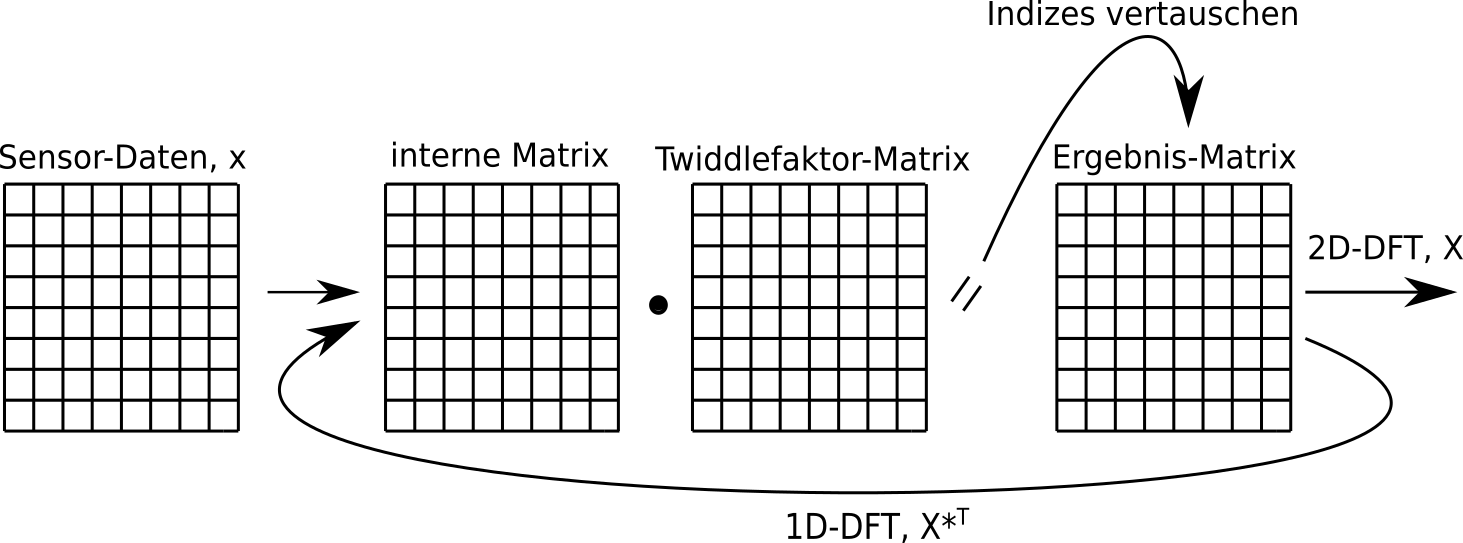
\includegraphics[width=0.95\textwidth]{img/MatMultTranspose2.png}
 \caption{Darstellung der Berechnung der 2D-DFT aus Gleichung (\ref{eq:MatMultTranspose2})}
 \label{pic:MatMultTranspose}
\end{figure}

\subsubsection{W = transpose(W)}

\subsection{Direkte Weiterverarbeitung der Zwischenergebnisse}
Um die Anzahl an Gattern und somit den Flächenbedarf zu reduzieren ist es das Ziel, die Ergebnisse der \gls{1d-dft} aus der 1. Berechnungsstufe im nächsten Schritt direkt als 
Eingangswerte für die \gls{2d-dft} zu verwenden. Auf diese Weise würden 64$\cdot$2$\cdot$12 Bit = 1536 Bit = 1,5kBit = 192 Byte an Speicher eingespart werden.
Wie sich im Laufe der Entwicklung gezeigt hat, lässt sich das nicht nutzen. Das liegt daran, dass dazu übergegangen wurde, immer nur ein Element zur Zeit berechnet wird und die 
bereits errechneten demnach zwischengespeichert werden müssen. Dieser Ansatz wurde verfolgt, da der Entwicklungsaufwand in VHDL für die spaltenweise Berechnung der Ausgangswerte 
einfacher umzusetzen war und es zunächst nur um die mathematische Umsetzung und nicht um die Platzeffizienz auf einem Chip ging.

Unklar war zu diesem Zeitpunkt noch, wie der Speicher realisiert werden soll. In der finalen Variante des Chips soll es einen \gls{ram} geben, der als zentraler
Speicher von allen Komponenten genutzt wird. Da die Entwicklung im Projekt noch nicht soweit fortgeschritten ist und dies nicht zu den Aufgaben der vorliegenden Arbeit gehört,
wurde auf das Speichern in lokalen Speicherzellen ausgewichen, welche als Variable oder Signal im VHDL-Code definiert und von der Software als Flip-Flop synthetisiert werden.



\subsection{Optimierte 8x8 DFT als Matrixmultiplikation}\label{sec:OptimierteMatrixmultiplikation}


Anfangs wurde angenommen, dass Multiplikationen mit den Twiddlefaktoren $\pm 1$ und $\pm\frac{\sqrt{2}}{2}$ durchgeführt werden müssen. 
Dass bei einer optimierten 8x8-DFT wegen des explizieten ausprogrammierens der Berechnungen die Multiplikation mit $\pm1$ wegfällt, wurde recht schnell klar.
Erst bei genauer Betrachtung der Twiddlefaktor-Matrix viel auf, dass in jeder Zeile gleich viele Additionen wie Subtraktionen vorhanden sind. Durch Umsortieren 
ist es dadurch möglich auf das Invertieren der Eingangswerte sowie den hierfür benötigten Takt und die Inverter zu verzichten. Weiter wird auch nur die Multiplikation
mit $+\frac{\sqrt{2}}{2}$ benötigt.

Anfangs wurde in Betracht gezogen das 1er-Komplement zu verwenden, da hierbei zwei betragsmäßig identische Zahen sich nur durch ihr höchstwertigstes 
 Bit unterscheiden. Auf diese Weise könnte das selbe Resultat für den Imaginär- wie für den Realteil verwendet werden, das Vorzeichen würde sich über eine 
 einfache XOR-Verknüpfung beider MSB der Multiplikanden ergeben.
 Diesem Vorteil steht jedoch eine aufwändigere Subtraktion (bzw. Addition negativer Zahlen) gegenüber. Der zusätzliche Aufwand entspricht 
 etwa dem der Bildung des 2er-Komplements. Aus diesem Grund und da das 2er-Komplement deutlich verbreiteter ist sowie weitere Vorteile bringt wie 
 beispielsweise keine Doppeldeutigkeit durch eine negative Null hat, wurde sich hierfür entschieden.
 
 
 In späteren Analysen konnte festgestellt werden, dass sowohl für den Real- als auch den Imaginärteil gleichviele Multiplikationen mit positiven wie mit negativen Faktoren 
 durchgefürht werden müssen. Dies lässt sich anhand des Einheitskreises in Abb. \ref{pic:Einheitskreis_Faktoren} und der Abbildung \ref{pic:Twiddlefaktoren_Darstellung8x8}
 nachvollziehen. Aus Abschnitt \ref{sec:Matrixmultiplikation} ist bekannt, dass bei einer Matrixmultiplikation Elemente multipliziert und anschließend die Ergebnisse 
 aufsummiert. Da es das Kommutativgesetz erlaubt die berechneten Ergebnisse auch in einer anderen Reihenfolge zu addieren, 

 
   
 In Abbildung \ref{pic:MatrizenDarstellungTwiddlefaktoren} ist zu sehen, dass die 2., 4., 6., und 8. Zeile je vier nicht triviale und komplexe Faktoren enthält. 
 Darüber hinaus ist ersichtlich, dass für komplexe Eingangswerte in den genannten Zeilen 12 und in den übrigen 8 Multiplikationen erfolgen müssen. Dies kann anhand der 
 Gleichungen (\ref{eq:komplexe_Multiplikation}) und (\ref{eq:halb_komplexe_Multiplikation}) nachvollzogen werden.
 Das lässt sich ausnutzen, um keine Negationen der Eingangs- und Zwischenwerte durchführen zu müssen. 
 

 
 Darüber hinaus
 minimiert sich bei geschickter Anordnung das Risiko eines Überlaufs. Wie in Abschnitt \ref{sec:NumerischeUngenauigkeiten} erwähnt, ist dies nicht Gegenstand dieser Arbeit,
 weshalb der Einfachheit wegen zur Sicherheit dennoch nach jeder Addition oder Subtraktion das Ergebnis durch einen Bitshift halbiert wird. 
 Es sei an dieser Stelle lediglich angemerkt, dass über die Eingangswerte die Annahme getroffen werden kann, dass aufeinanderfolgende Werte das selbe Vorzeichen haben. 
 Dies ließe sich ausnutzen, um noch weiter die Wahrscheinlichkeit zu reduzieren, dass es zu einem Überlauf kommt. 
 


% Später wohl besser ins Kapitel Entwicklung
Dies hat zur Folge, dass ein sehr großer Wert entstehen kann, welcher Maßgebend für die Anzahl der Vorkommabits sein kann.
%
Wegen der Null im Imaginärteil der ersten Zeile der Twiddlefaktormatrix sind auch alle Imaginärteile der ersten Spalte der Ausgangsmatrix Null.
Bezogen auf den Imaginärteil gilt das Gleiche auch für die fünfte Zeile der Twiddlefaktormatrix. 
%
Da sich beim Realteil der fünften Zeile der Twiddlefaktormatrix der fünften Zeile positive und negative Einsen abwechseln, sind hier auch keinerlei Multiplikationen nötig.

Aus der anfänglichen Implementation bei der alle nicht trivialen Werte einer Berechnung die entweder mit $+\frac{\sqrt{2}}{2}$ oder $-\frac{\sqrt{2}}{2}$ multipliziert wurden,
einzelnd berechnet werden, wird mittels des Distributivgesetzes der gemeinsame Faktor ausgeklammert, sodass nur noch jeweils eine Multiplikation erforderlich ist.


Bei den weiteren Zeilen sind hingegen die Zahlen zur Hälfte positiv und zur anderen negativ. Außerdem enthalten die geraden Zeilen den Faktor $\pm\frac{\sqrt{2}}{2}$. 
Dies lässt sich ausnutzen, um die Anzahl der der Multiplikationen zu reduzieren. Zunächst können die 

Für jede gerade Zeile der DFT ist jeweils für den Real- und den Imaginärteil eine Multiplikation nötig, so dass sich insgesamt acht Multiplikationen ergeben
 




 
 
\subsection{Berechnungsschema der geraden und ungeraden Zeilen}\label{sec:Berechnungsschema}

In Abbildung \ref{pic:AkkumulationUngeradeSpalten} ist die Berechnung der ungeraden Zeilen am Beispiel der ersten zu sehen.

\begin{figure}[htbp]
\centering
$a_{0} + a_{1} + a_{2} + a_{3} + a_{4} + a_{5} + a_{6} + a_{7}$\\

\vspace{0.5cm}
\begin{tabular}{ccccccccc}
Takt&\multicolumn{6}{l}{ } & & Bit\\
1&$\underbrace{a_{k0} + a_{k1}}$ &  &$ \underbrace{a_{k2} + a_{k3}}$ &  &$\underbrace{a_{k4} + a_{k5}}$ &  &$\underbrace{a_{k6} + a_{k7}}$ & 12\\
&\multicolumn{7}{l}{$\hspace{0.65cm} \Downarrow \hspace{2.3cm} \Downarrow \hspace{2.3cm} \Downarrow \hspace{2.3cm}\Downarrow$}&13\\
2&\multicolumn{3}{c}{$\underbrace{sum\_1\_1 \quad + \quad sum\_1\_2}$} & & \multicolumn{3}{c}{$\underbrace{sum\_1\_3 \quad + \quad sum\_1\_4}$} & 12\\
&\multicolumn{3}{c}{$\Downarrow$} & & \multicolumn{3}{c}{$\Downarrow$}&13\\
3&\multicolumn{7}{c}{$\underbrace{sum\_2\_1 \quad  \quad \quad \quad + \quad \quad \quad  \quad sum\_2\_2}$} & 12\\
&\multicolumn{7}{c}{$\Downarrow$}&13\\
&\multicolumn{7}{c}{$sum\_3\_1$} & 12\\
&\end{tabular}
%\captionof{figure}{Vorgehensweise der Akkumulation der ungeraden Spalten der Eingangswerte}
\caption{Vorgehensweise der Akkumulation der ungeraden Spalten der Eingangswerte.}
\label{pic:AkkumulationUngeradeSpalten}
\end{figure}
%\end{center}

\vspace{0.5cm}

Wie der linken Spalte zu entnehmen ist, werden 3 Takte für die Berechnungen der Werte aus den ungeraden Spalten der Eingangsmatrix bzw. ungeraden Zeilen der 1D-DFT-Matrix benötigt.
1. Takt für Additionen bzw. Subtraktionen und 2. sowie 3. Takt für das Aufsummieren. Der Bitvektor des Ergebnisses ist zwar 12 Bit breit, aber beim letzten Bitshift von 13 auf 12
werden nur 11 Bit übernommen. Es wird alo ein doppelter Bitshift vollzogen. Dies erfolgt, damit sowohl in den geraden als auch den ungeraden Zeilen gleich viele Bitshifts erfolgen
und die Werte somit identisch skaliert sind.

Die Berechnung der geraden Zeilen wird in Abbildung \ref{pic:AkkumulationGeradeSpalten} am Beispiel der zweiten Zeile gezeigt
\begin{figure}[htbp]
 \centering
 $a_0 - x_1 + x_0 - b_2 + x_2 - x_3 + a_4 - x_5 + x_4 - b_6 + x_6 - x_7$\\

 \vspace{0.3cm}
 
\begin{tabular}{ccccccccccccc}
Takt&\multicolumn{11}{c}{}&Bit\\
1 &$\underbrace{a_0 - x_1}$ &        &$ \underbrace{x_0 - b_2}$ &  &$\underbrace{x_2 - x_3}$ &  &$\underbrace{a_4 - x_5}$ &  &$\underbrace{x_4 - b_6}$ &$\underbrace{x_6 - x_7}$& &12\\
  &\multicolumn{11}{l}{$\hspace{0.5cm} \Downarrow \hspace{1.75cm} \Downarrow \hspace{2.4cm} \Downarrow \hspace{1.8cm}\Downarrow \hspace{1.8cm}\Downarrow \hspace{1.4cm}\Downarrow$}&13\\
2 &\multicolumn{3}{c}{$\underbrace{sum1\_1 \: + \: sum1\_2}$} & & \multicolumn{3}{c}{$\underbrace{sum1\_3 \: + \: sum1\_4}$} &\multicolumn{3}{c}{$\: \underbrace{sum1\_5 \: + \: sum1\_6}$}& &12\\
  &\multicolumn{3}{c}{$\Downarrow$}  & & \multicolumn{3}{c}{$\Downarrow$} & & \multicolumn{2}{c}{$\Downarrow$}& &13\\
3 &\multicolumn{7}{c}{$\underbrace{sum2\_1 \quad  \quad \quad \quad + \quad \quad \quad  \quad sum2\_2}$} & & & & &12\\
  &\multicolumn{7}{c}{$\Downarrow$}& & \multicolumn{2}{c}{$\Downarrow$}& &13\\
  &\multicolumn{7}{c}{$sum3\_1$}& & & & &13\\
  & & & & $\Downarrow$& & & & & \multicolumn{2}{c}{$\Downarrow$} & & 13\\
4 & & & & $\frac{\sqrt{2}}{2}$&\multicolumn{5}{c}{}& & &13\\
  & & & & $\Downarrow$& & & & & \multicolumn{2}{c}{$\Downarrow$ }& & 26\\
5 & & & \multicolumn{9}{c}{$\underbrace{sum4\_1 \:  \quad \quad \quad \quad \quad \quad + \quad \quad \quad \quad \quad \quad   sum2\_3}$} &12\\
  & & & \multicolumn{9}{c}{$\Downarrow$}&13\\
  & & & \multicolumn{9}{c}{$sum5\_1$}&12\\
\end{tabular}
\caption{Vorgehensweise der Akkumulation der geraden Spalten der Eingangswerte.}
\label{pic:AkkumulationGeradeSpalten}
\end{figure}

\vspace{1cm}
Auch hier ist der linken Spalte die Anzahl der benötigten Takte zu entnehmen. In diesem Fall werden 5 Takte für die Berechnungen benötigt. Diese setzen sich zusammen aus
1 Takt für Additionen bzw. Subtraktionen, 2.-3. sowie 5. Takt für das Aufsummieren und der 4. Takt für die Multiplikationen.

Wie rechts am Rand zu sehen, ergibt sich durch die Addition eine Bitbreitenerweiterung um 1 bzw. bei der Multiplikation eine Verdoppelung. Bei einer früheren 
Implementierung, die nur die 1D-DFT beherrschte, wurde zumindest die Erweiterung bei der Addition umgesetzt. Da bei der 2D-DFT die selbe Recheneinheit genutzt 
werden soll, wurde in Absprache mit dem ISAR-Team entschieden, dass die Summanden vor jeder Summation durch einen Bitshift nach rechts halbiert werden. Auf diese
Weise hat ein Additionsergebnis immer 13 Bit Breite. Durch den Bitshift kann das Resultat der 1D-DFT direkt als Eingang für die 2D-DFT verwendet werden. 

Zu bedenken gilt es bei einem Bitshift, dass das Ergebnis mit jedem Mal eine Division durch 2 erfährt. Bei hintereinander erfolgenden Bitshifts wird demnach durch $2^{N_B}$ geteilt, 
wobei $N_B$ die Anzahl der Bitshifts ist. Den beiden obigen Darstellungen der Summationen kann entnommen werden, dass, um ein Überlaufen des Bitvektors zu vermeiden es nötig ist,
drei respektive vier Bitshifts durch zu führen. Wie bereits erläutert erfolgt bei den ungeraden Zeilen abschließend ein doppelter Bitshift. Auf diese Weise ergibt sich für die
1D-DFT, dass das Ergebnis um den Faktor 16 kleiner ist, als beispielsweise bei der Berechnung mit Matlab. Da bei bei dem zweiten Durchlauf, um die 2D-DFT zu berechnen, ebenfalls 
durch 16 geteilt wird, ergibt sich insgesamt eine Division durch $2^{2\cdot4} = $ 256.

\subsubsection{Erwartete Anzahl benötigter Takte}
Aus den Abbildungen \ref{pic:AkkumulationUngeradeSpalten} und \ref{pic:AkkumulationGeradeSpalten} können die Takte die zur Berechnung der 1D- bzw. 2D-DFT benötigt werden 
abgeleitet werden.

Für ungeraden Zeilen sind je Element 3 Takte nötig und mit 8 Elementen pro Zeile und 4 ungeraden Zeilen errechnen sich so 3$\cdot$8$\cdot$4=96 Takte.
Analog errechnet sich für die ungeraden Zeilen mit je 5 Takten pro Element 5$\cdot$8$\cdot$4=160 Takte.
In der Summe ergeben sich so 96+160=256 Takte für die 1D-DFT. Da die 2D-DFT ohne Takte fürs Umspeichern oder ähnliches sofort im Anschluss berechnet werden kann, 
verdoppelt sich die Anzahl der Takte auf 512 für die vollständige Berechnung.




\subsubsection{Zusammenhang von DFT und IDFT bei der Matrixmultiplikation}

Durch die umgekehrte Drehrichtung des komplexen Zeigers in Gleichung (\ref{eq:idft}) werden in der Matrizenschreibweise die Zeilen 2 und 8, 3 und 7 sowie 4 und 6 vertauscht.
Nachvollziehen lässt sich das gut anhand der Grafik (\ref{pic:Einheitskreis_Faktoren}). 
Verdeutlicht wird das vorgehen in Abbildung \ref{pic:IDFT_Zeilentausch}.

\begin{figure}[ht]
 \centering
 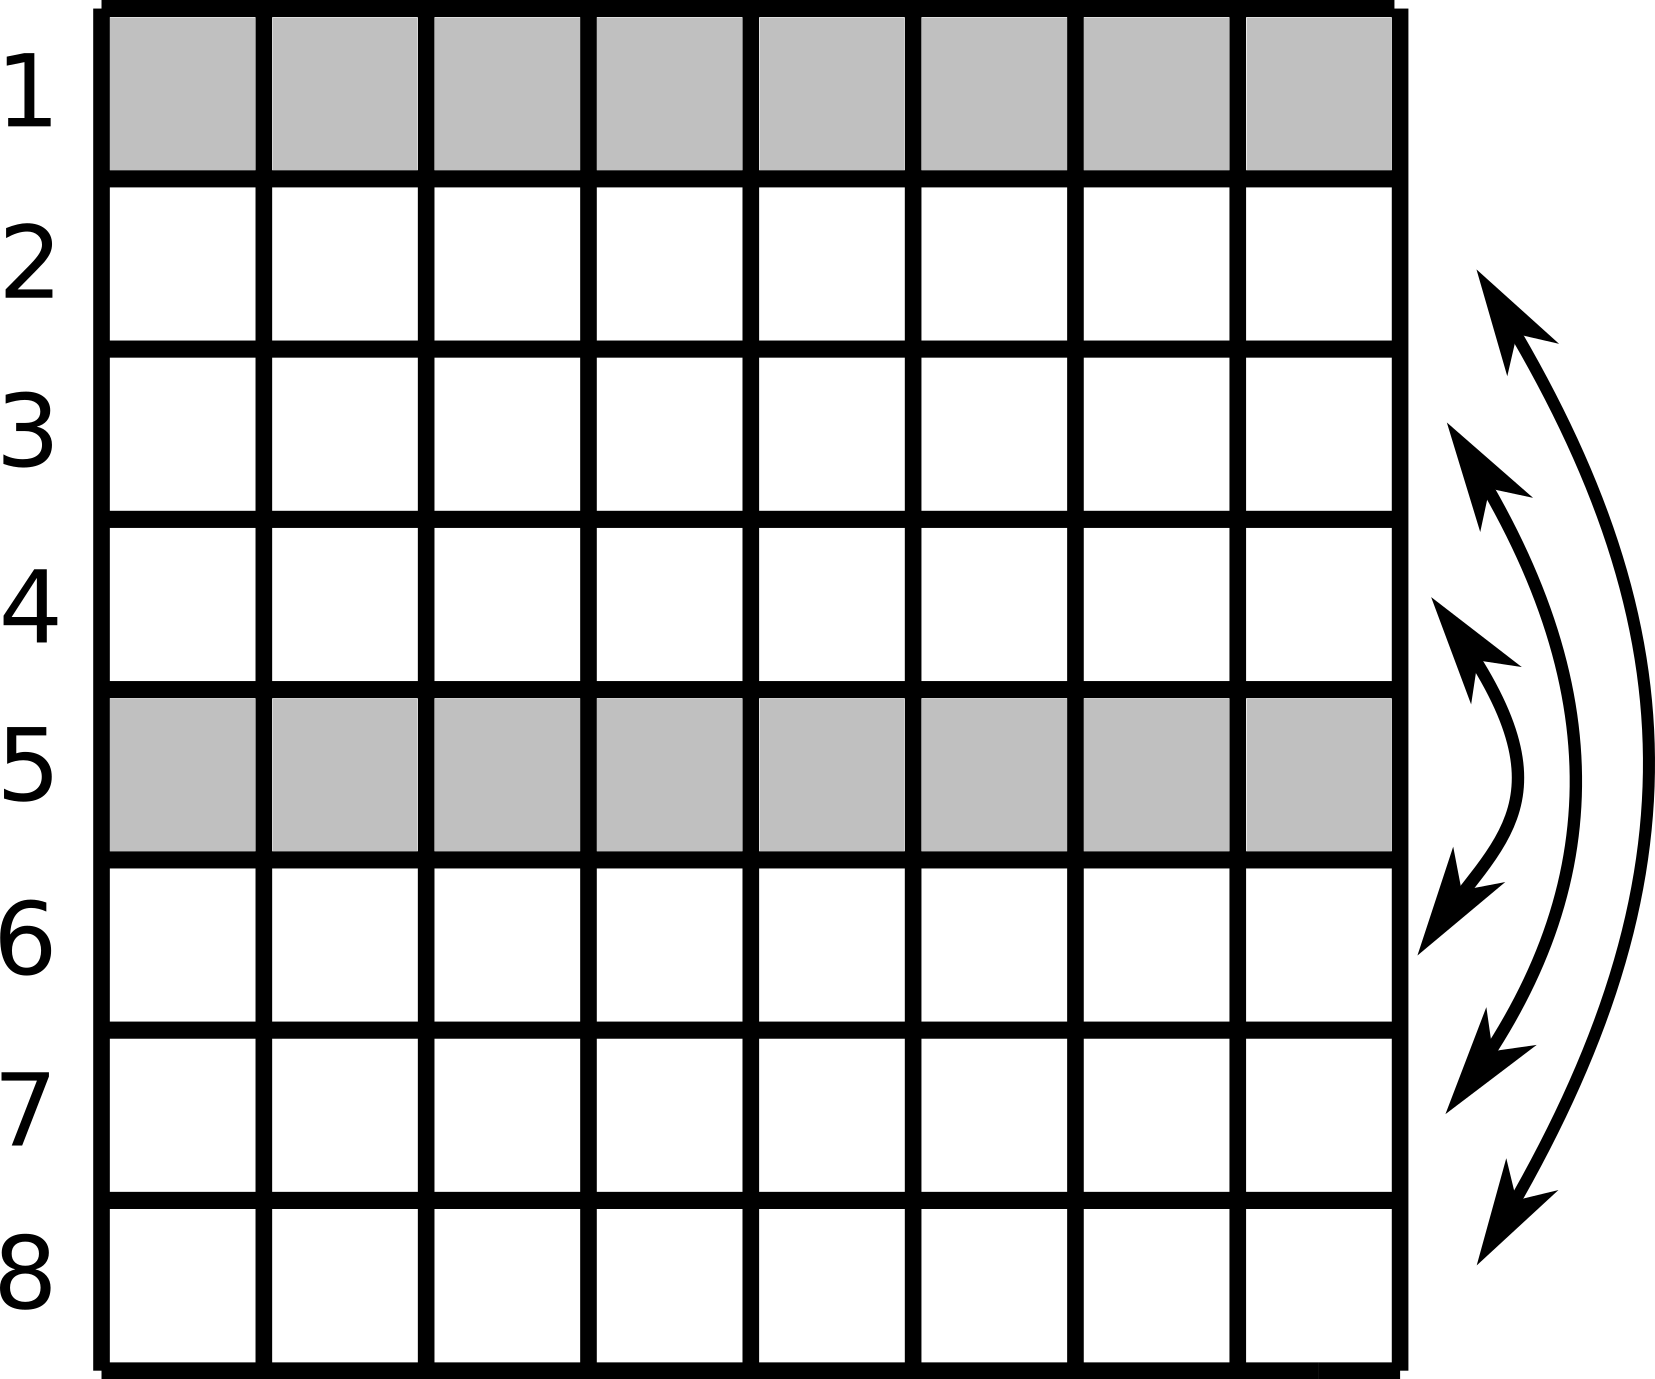
\includegraphics[width=0.4\textwidth]{img/IDFT_Zeilentausch.png}
 \caption{Um von der DFT zur IDFT zu kommen, müssen bei der Matrixmultiplikation die Zeilen 2 und 8, 3 und 7 sowie 4 und 6 der Twiddlefaktormatrix vertauscht werden.}
 \label{pic:IDFT_Zeilentausch}
\end{figure}



\subsection{Test der Matrixmultiplikation}


\subsubsection{1D-DFT mit Integer-Werten}
 
\subsubsection{2D-DFT mit Integer-Werten}

\subsubsection{2D-DFT mit Werten SQ-Format}

Unter anderem weil NC\,Sim bzw. dessen Unterprogramm SimVision zur Anzeige von Signalverläufen (Waveform) nur Integer darstellen kann und bei als Vektor gebündelten Signalen 
diese nicht einmal als vorzeichenbehaftet (signed), wurde der Einfachheit halber zunächst die Berechnung als Ganzzahl-Multiplikation mit dem Faktor 3 betrachtet. 
Da es bei diesem Faktor und den gewählten Eingangswerten nicht zu einem 
Überlauf kommen kann, war es zu diesem Zeitpunkt noch nicht nötig, sich Gedanken über die Breite des Ergebnisvektors bzw. den Ausschnitt daraus für die weitere
Berechnung zu machen. Deshalb konnte an dieser Stelle noch auf den Bitshift zur Halbierung der Werte verzichtet werden.

Erst als der Faktor $\frac{\sqrt{2}}{2}$ übernommen wurde, wurden die Ergebnisse breiter als der Vektor für die weitere Berechnung an Bits zur Verfügung stellt.

${\frac{\sqrt{2}}{2}}_{10}$ = $0001011010100_2$ in S2Q10, als Integer betrachtet jedoch $724_{10}$.

Daraus folgt, dass ein Teil der Bits abgeschnitten werden müssen. Da die Dualzahlen jetzt im S1Q10-Format betrachtet werden, es sich also um Kommazahlen handelt,
müssen die hinteren Bits abgeschnitten werden. Zudem können vorne Bits ohne Informationsverlust gestrichen werden, da durch die Multiplikation ein weiteres 
Negations-Bit dazugekommen ist und auf Grund des gegebenen Faktors der Wertebereich vorne nie ganz ausgenutzt wird. (Verifizieren / Belegen!)



\section{Syntheseergebnisse von Teilkomponenten}\label{sec:Syntheseergebnisse}
\subsection{13 Bit Konstantenmultiplizierer}\label{sec:Konstantenmultiplizierer}

Der duale Wert lässt sich am einfachsten mit der Matlab-Funktion \texttt{fi()} ermitteln. Der Funktion werden hierfür Kommagetrennt der Deziamlwert, 1 für vorzeichenbehaftet,
die gesamte Anzahl an Stellen (13) und die Anzahl der Nachkommastellen (10) übergeben. Der vollständige Aufruf sieht dann wie folgt aus:

\texttt{val=fi(sqrt(2)/2,1,13,10)}

Der erzeugte Datentyp hat unter anderem die Eigenschaften \texttt{val.bin}, welche einem mit $0001011010100$ den Wert als Binärzahl zurück gibt, 
\texttt{val.double} gibt den approximierten Dezimalwert mit 0,70703125 zurück und \texttt{val.dec} interpretiert den Dualwert als Integer, was 724 entspricht.
Letzterer ist wichtig zu kennen, um die Werte der Simulation nachvollziehen zu können.

Der Berechnung aus Gleichung (\ref{eq:abweichungWurzel2halbe}) kann entnommen werden, dass die Abweichung weit unter einem Prozent liegt.

\begin{equation}\label{eq:abweichungWurzel2halbe}
 \frac{100}{\dfrac{\sqrt{2}}{2}}\cdot 0,70703125 = 99,989\%
\end{equation}

Zeigen, welche Bits heraus genommen werden müssen! und belegen warum.

\begin{figure}[!ht]
\centering  
 %\fbox{
  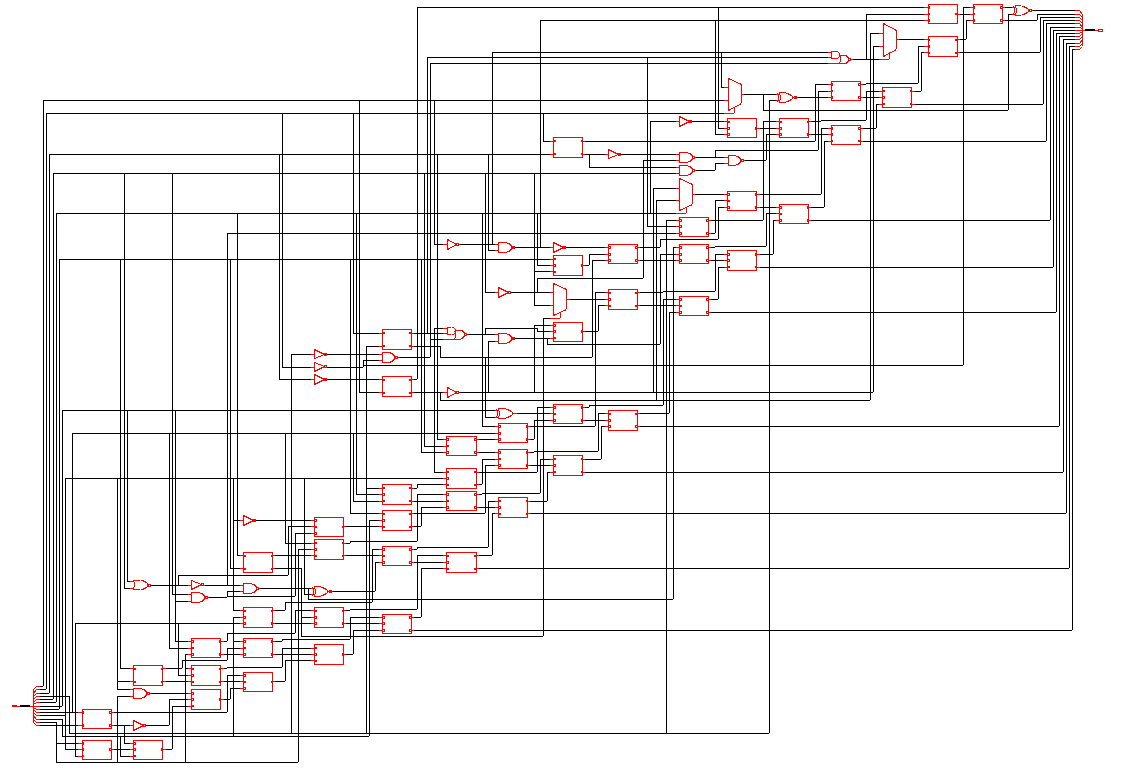
\includegraphics[width=1\textwidth]{img/13Bit_Konstantenmultiplizierer_neu.png}
  %}
  \caption{Schaltnetz des 13 Bit Konstantenmultiplizierers für $\frac{\sqrt{2}}{2} = 0.70711 \simeq 0.70703125 = 0001011010100_2$ in Encounter; Eingang links, Ausgang rechts}
  \label{pic:Konstantenmultiplizierer}
\end{figure}

Der vollständige Gate-Report befindet sich in Abschnitt \ref{src:rc_gate_report} auf Seite \pageref{src:rc_gate_report}



\subsection{Bildung des 2er-Komplements eines 13 Bit Vektors}


In Abb. \ref{pic:13BitInverter} ist die nicht expliziet implementierte, aber in Abschnitt \ref{sec:RelleEingangswerte} erwähnte Negierung von Zahlen zu sehen.

\begin{figure}[htpb]
\centering
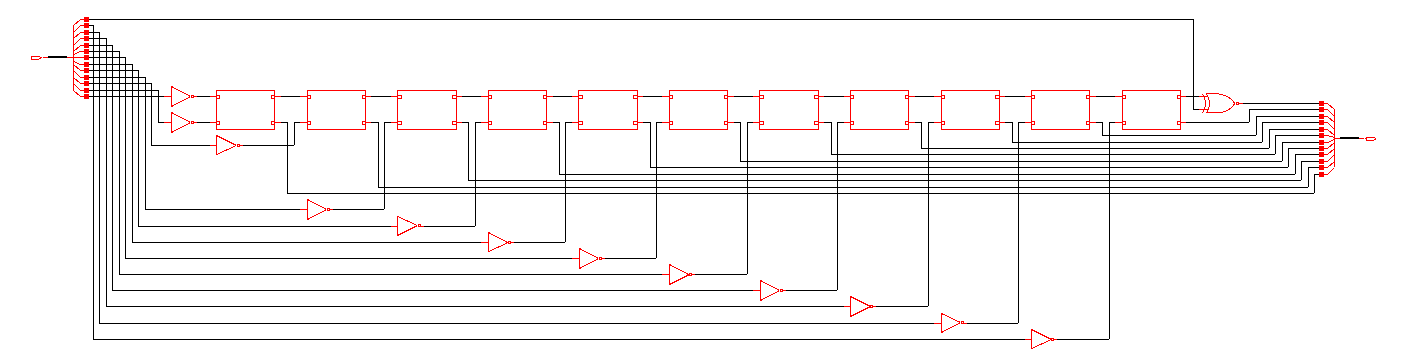
\includegraphics[width=0.99\textwidth]{img/13Bit_Negierer.png}
\caption{Schaltnetz einer Einheit zur Bildung des 2er-Komplements eines 13 Bit Vektors; Eingang links, Ausgang rechts}
\label{pic:13BitInverter}
\end{figure}

Für die Negierung eines 13 Bit Vektors hat das Synthesewerkzeug \texttt{encounter} 22 Standardzellen verwendet. Das sind knapp doppelt so viele Gatter, wie der Vektor 
Bits breit ist. Der Unterschied zum Konstantenmultiplizierer fällt somit sehr gering aus. 
Wie zu sehen, handelt es sich fast ausschließlich um Inverter und Addierer. In Abschnitt \ref{sec:Integer2erKomplement} wurde bereits beschrieben, dass für die Bildung des
2er-Komplements zunächst alle Bits invertiert werden müssen. Abschließend wird auf den Vektor 1 LSB addiert. 
Beide Pfade weisen die gleiche Länge auf und verwenden überwiedend die selben
Gattertypen, weshalb darauf geschlossen werden kann, dass die maximale Gatterlaufzeit in der gleichen Größenordnung liegen muss.

\subsection{13 Bit Addierer}
Der 13 Bit Addierer hat zwei 13 Bit Eingänge, allerdings werden durch einen Bitshift beide Eingangswerte halbiert, damit kein Überlauf entsteht. Insofern fließen nur jeweils 
die forderen 12 Bit in die Berechnung ein.
\begin{figure}[htbp]
 \centering
 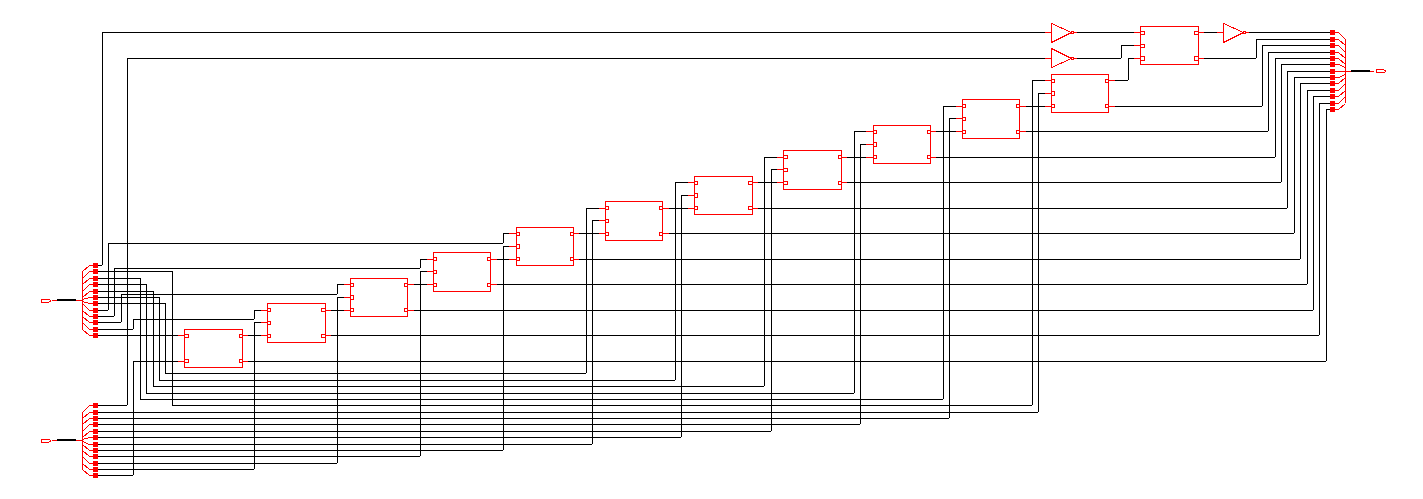
\includegraphics[width=0.99\textwidth]{img/13Bit_Addierer.png}
 \caption{Schaltnetz eines 12 Bit Addierers, Eingänge links (12\,Bit), Ausgang rechts (13\,Bit)}
 \label{pic:13BitAddierer}
\end{figure}

\subsection{Vergleich der Syntheseergebnisse}
 In Tabelle \ref{tab:VergleichSyntheseergebnisse} ist eine Gegenüberstellung der Syntheseergebnisse unter den Aspekten Anzahl der Gatter und Fläche.
\begin{table}[!ht]
\centering
 \caption{Vergleich}
 \label{tab:VergleichSyntheseergebnisse}
 \begin{tabular}{lcc}
 \hline
				&Gatter  	&Fläche (Prozess: 350nm) \\
  \hline	
  13\,Bit Konstantenmultiplizierer für $\nicefrac{\sqrt{2}}{2}$	& 82		& $\SI{6612}{\um^2}$ \\
  13\,Bit regulärer Multiplizierer				& 175		& $\SI{23261}{\um^2}$\\
  12\,Bit Addierer						& 15		& $\SI{3257}{\um^2}$\\
  13\,Bit 2er-Komplement-Bildung				& 24		& $\SI{2147}{\um^2}$\\
  \hline
 \end{tabular}
\end{table}



\subsubsection{Gegenüberstellung der Konstantenmultiplikation und der Bildung des 2er-Komplements}

Unter diesem Punkt sollen die Konstantenmultiplikation und die Bildung des 2er-Komplements unter Aspekten der benötigten Zeit und des benötigten Platzes auf einem Chip 
betrachtet werden. Um einen Eindruck hiervon zu erhalten, werden im Kapitel Entwurf in Abschnitt \ref{sec:Syntheseergebnisse} jeweils die Schaltnetzte 
%für die Negation mittels 2er-Komplement und die Multiplikation mit einem konstanten Faktor 
gezeigt.
Wie dort erläutert, lässt sich anhand dieser sagen, dass es bei dieser Art der Implementierung keinen zeitlichen Gewinn gibt, da beide kritischen Pfade etwa gleich lang 
sind. Für die knapp $4$ mal mehr Gatter bei der Multiplikation ist auch ein größerer Vertrahtungsaufwandt erforderlich, sodass die Konstantenmultiplizierer
auf einem Chip eine etwas größere Fläche beanspruchen. Da es sich hier insgesamt aber um wenige Gatter handelt, wirkt sich dies erst bei sehr vielen Instanzen aus.
Es kann an dieser Stelle deshalb festgehalten werden, dass dieser Unterschied nicht als entscheidend geltend gemacht werden kann.
